\section{Cyclic Codes}
In this section, we have three goals:
\begin{enumerate}[(1)]
	\item To understand the ideal correspondence between a ring $R$ and its quotient
	\[
	R \longrightarrow R/I.
	\]
	
	\item To interpret this correspondence geometrically through spectra, first in the familiar examples
	\[
	\Z \qquad\text{and}\qquad \C[x].
	\]
	
	\item To apply the same idea to the quotient ring
	\[
	\F_q[x]/\ideal{x^n-1}
	\]
	and explain why its ideals are exactly the cyclic codes of length $n$ over $\F_q$.
\end{enumerate}

The central philosophy is the following:

\begin{quote}
	Passing from $R$ to $R/I$ means forcing the elements of $I$ to become zero.  
	Therefore only those ideals of $R$ that already contain $I$ survive in the quotient.
\end{quote}

In the cyclic-code setting, the additional feature is that the quotient ring
\[
\F_q[x]/\ideal{x^n-1}
\]
is naturally identified with the vector space $\F_q^n$, and multiplication by $x$ becomes cyclic shift of coordinates. This turns ring-theoretic ideals into coding-theoretic cyclic codes.

\newpage
\subsection{The ideal correspondence for a quotient ring}
\thmbox[Ideal Correspondence]{\begin{theorem}\label{thm:ideal-correspondence}
	Let $R$ be a ring, let $I \triangleleft R$ be an ideal, and let
	\[
	\pi:R\longrightarrow R/I
	\]
	be the quotient map. Then the assignment
	\[
	J' \longmapsto \pi^{-1}(J')
	\]
	defines an inclusion-preserving bijection
	\[
	\{\text{ideals of }R/I\}
	\longleftrightarrow
	\{\text{ideals }J\triangleleft R \text{ such that } I\subseteq J\}.
	\]
	Its inverse is given by
	\[
	J \longmapsto J/I.
	\]
\end{theorem}}


\begin{proof}
	Let $J' \triangleleft R/I$. Then $\pi^{-1}(J')$ is an ideal of $R$. Since $\pi(I)=0$, we have
	\[
	I \subseteq \pi^{-1}(J').
	\]
	
	Conversely, let $J \triangleleft R$ with $I\subseteq J$. Then
	\[
	J/I=\{\ol{x}\in R/I : x\in J\}
	\]
	is an ideal of $R/I$.
	
	Now we check that these constructions are inverse to one another.
	
	If $J \triangleleft R$ with $I\subseteq J$, then
	\[
	\pi^{-1}(J/I)=J.
	\]
	Indeed, $\pi(x)\in J/I$ if and only if $x\in J$.
	
	If $J' \triangleleft R/I$, then
	\[
	\pi^{-1}(J')/I=J'.
	\]
	Indeed, every element of $J'$ has the form $\ol{x}$ with $x\in \pi^{-1}(J')$.
	
	Thus the correspondence is bijective, and it is plainly inclusion-preserving. 
\end{proof}

\begin{remark}
	This theorem says \[
	\text{ideals of }R/I
	\quad\leftrightarrow\quad
	\text{ideals of }R\text{ containing }I.
	\]
\end{remark}

\newpage

\subsection{Cyclic codes as ideals}
%\begin{definition}
%	Let \(n\ge 1\), and let \(\F_q\) be the finite field with \(q\) elements. A \emph{linear code of length \(n\) over \(\F_q\)} is an \(\F_q\)-linear subspace
%	\[
%	C\le \F_q^n.
%	\]
%	If \(\dim_{\F_q}C=k\), then \(C\) is called an \emph{\([n,k]_q\)-code}.
%\end{definition}
\begin{observation}
Consider the code \[
\code=\set{\texttt{000},\texttt{011},\texttt{101},\texttt{110}}\leq\F_2^3.
\] Under the isomorphism \[
\fullfunction{\Phi}{\F_2^3}{\F_2[x]/\ideal{x^3-1}}{(c_0,c_1,c_2)}{c_0+c_1x+c_2x^2},
\] the cyclic shift of coordinates corresponds to multiplication by \(x\) modulo \(x^3-1\). 	\[
\begin{array}{c|c|c}
	\text{Codeword} & \text{Vector} & \text{Polynomial} \\
	\hline
	\texttt{000} & (0,0,0) & 0 \\
	\texttt{011} & (0,1,1) & x+x^2 \\
	\texttt{101} & (1,0,1) & 1+x^2 \\
	\texttt{110} & (1,1,0) & 1+x \\
\end{array}
\] So in polynomial form, \[
\code=\set{0,x+x^2,1+x^2,1+x}\subseteq \F_2[x]/\ideal{x^3-1}.
\] Now observe that \[
x^3-1=x^3+1=(x+1)(x^2-x+1)=(x+1)(x^2+x+1)
\] in $\F_2[x]$. \begin{center}
	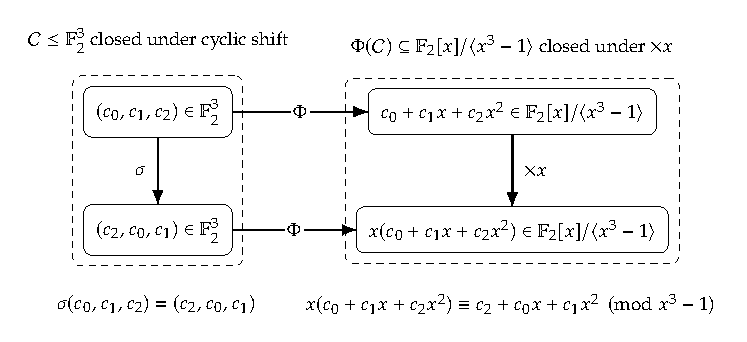
\includegraphics[scale=1.25]{tikz/cyclic-code-2.pdf}
\end{center}
%The essential point is that cyclic shift in \(\F_2^3\) becomes multiplication by \(x\) in \(\F_2[x]/\ideal{x^3-1}\). Since \(\code\) is an \(\F_2\)-linear subspace closed under cyclic shift, its image under \(\Phi\) is closed under multiplication by \(x\), hence by every polynomial in \(x\), and therefore is an ideal of the quotient ring.
\end{observation}

\newpage
\defbox[Cyclic code]{\begin{definition}
	A linear code \(\code\le \F_q^n\) is called a \textbf{cyclic code} if \[
	c=(c_0,c_1,\dots,c_{n-1})\in\code\implies c^{\ggg 1}=(c_{n-1},c_0,c_1,\dots,c_{n-2})\in\code.
	\] In other words, the cyclic shift of every codeword is also a codeword.
\end{definition}}
\begin{remark}
	Consider the cyclic shift operator
	\[
	T:\F_q^n\to \F_q^n,\qquad
	T(c_0,c_1,\dots,c_{n-1})=(c_{n-1},c_0,c_1,\dots,c_{n-2}),
	\] Then \(\code\) is cyclic if and only if $T(\code)=\code$. Thus a cyclic code is a linear subspace of \(\F_q^n\) invariant under cyclic shift.
\end{remark}



%\begin{remark}
%	If a cyclic code \(C\) has dimension \(k\) and minimum Hamming distance \(d\), then \(C\) is called an \emph{\([n,k,d]_q\)-cyclic code}.
%\end{remark}

\medskip
\thmbox[Cyclic codes are Ideals]{\begin{theorem}
Identify \(\F_q^n\) with the quotient ring \(\F_q[x]/\ideal{x^n-1}\) by
\[
(c_0,c_1,\dots,c_{n-1})
\longleftrightarrow
c_0+c_1x+\cdots+c_{n-1}x^{n-1}\pmod{x^n-1}.
\]
Under this identification, a linear code \(C\le \F_q^n\) is cyclic if and only if the corresponding subset is an ideal of
\[
\F_q[x]/\ideal{x^n-1}.
\]
\end{theorem}}
\begin{proof}
	Under the above identification, multiplication by \(x\) in \(\F_q[x]/\ideal{x^n-1}\) sends
	\[
	c_0+c_1x+\cdots+c_{n-1}x^{n-1}
	\]
	to
	\[
	c_{n-1}+c_0x+c_1x^2+\cdots+c_{n-2}x^{n-1},
	\]
	because \(x^n\equiv 1\pmod{x^n-1}\). This is exactly the cyclic shift
	\[
	(c_0,c_1,\dots,c_{n-1})
	\mapsto
	(c_{n-1},c_0,c_1,\dots,c_{n-2}).
	\]
	
	Hence a linear subspace \(C\le \F_q^n\) is closed under cyclic shift if and only if the corresponding subset of \(\F_q[x]/\ideal{x^n-1}\) is closed under multiplication by \(x\). Since it is already closed under addition and scalar multiplication, this is equivalent to being an ideal.
\end{proof}


\begin{example}[The ideal lattice of \texorpdfstring{$\F_2[x]/\ideal{x^3-1}$}{F2[x]/(x^3-1)} and the corresponding cyclic codes]
	Let
	\[
	A=\F_2[x]/\ideal{x^3-1}.
	\]
	Since in \(\F_2[x]\) we have
	\[
	x^3-1=x^3+1=(x+1)(x^2+x+1),
	\]
	the monic divisors of \(x^3-1\) are
	\[
	1,\qquad x+1,\qquad x^2+x+1,\qquad x^3+1.
	\]
	Therefore the ideals of \(A\) are exactly
	\[
	\ideal{\ol{1}},\qquad
	\ideal{\ol{x+1}},\qquad
	\ideal{\ol{x^2+x+1}},\qquad
	\ideal{\ol{x^3+1}}=\ideal{\ol{0}}.
	\]
	The ideal lattice is therefore
	\[
	\begin{tikzcd}[row sep=large, column sep=large]
		& \ideal{\ol{1}}=A \arrow[dl] \arrow[dr] & \\
		\ideal{\ol{x+1}} \arrow[dr] & & \ideal{\ol{x^2+x+1}} \arrow[dl] \\
		& \ideal{\ol{0}} &
	\end{tikzcd}
	\]
	
	We now describe the corresponding cyclic codes under the identification
	\[
	(c_0,c_1,c_2)\longleftrightarrow c_0+c_1x+c_2x^2
	\]
	between \(\F_2^3\) and \(A\).
	
	\begin{enumerate}
		\item The ideal
		\[
		\ideal{\ol{1}}=A
		\]
		corresponds to the whole space
		\[
		\F_2^3
		=
		\{000,001,010,011,100,101,110,111\}.
		\]
		
		\item The ideal
		\[
		\ideal{\ol{x+1}}
		\]
		is generated by \(x+1\). Its elements are
		\[
		0,\qquad x+1,\qquad x(x+1)=x^2+x,\qquad x^2(x+1)=x^3+x^2\equiv 1+x^2
		\pmod{x^3-1}.
		\]
		Thus
		\[
		\ideal{\ol{x+1}}
		=
		\{\,0,\ x+1,\ x^2+x,\ 1+x^2\,\}.
		\]
		In vector form, this is
		\[
		\{000,110,011,101\}
		=
		\{000,011,101,110\}.
		\]
		This is the even-weight code of length \(3\).
		
		\item The ideal
		\[
		\ideal{\ol{x^2+x+1}}
		\]
		is generated by \(x^2+x+1\). Since
		\[
		x(x^2+x+1)=x^3+x^2+x\equiv 1+x^2+x=x^2+x+1
		\pmod{x^3-1},
		\]
		multiplication by \(x\) does not produce a new element. Hence
		\[
		\ideal{\ol{x^2+x+1}}
		=
		\{\,0,\ x^2+x+1\,\}.
		\]
		In vector form, this is
		\[
		\{000,111\},
		\]
		the repetition code of length \(3\).
		
		\item The ideal
		\[
		\ideal{\ol{0}}
		\]
		corresponds to the zero code
		\[
		\{000\}.
		\]
	\end{enumerate}
	
	Therefore the four cyclic codes of length \(3\) over \(\F_2\) are exactly
	\[
	\F_2^3,\qquad
	\{000,011,101,110\},\qquad
	\{000,111\},\qquad
	\{000\}.
	\]
	
	Their inclusion lattice is
	\[
	\begin{tikzcd}[row sep=large, column sep=large]
		& \F_2^3 \arrow[dl] \arrow[dr] & \\
		\{000,011,101,110\} \arrow[dr] & & \{000,111\} \arrow[dl] \\
		& \{000\} &
	\end{tikzcd}
	\]
	
	Notice that the two middle codes are incomparable:
	\[
	111\notin \{000,011,101,110\},
	\qquad
	110\notin \{000,111\}.
	\]
	Thus the lattice has the shape of a diamond.
	
	This example illustrates the general principle: cyclic codes correspond to the ideals of
	\[
	\F_q[x]/\ideal{x^n-1},
	\]
	and these ideals are classified by the divisors of \(x^n-1\).
\end{example}

\newpage
\begin{remark}
	The appearance of ideals containing \((x^n-1)\) comes from the correspondence theorem for ideals. Indeed, cyclic codes are first identified with ideals of the quotient ring
	\[
	\F_q[x]/(x^n-1).
	\]
	If
	\[
	\pi:\F_q[x]\to \F_q[x]/(x^n-1)
	\]
	is the quotient map, then every ideal of \(\F_q[x]/(x^n-1)\) is of the form \(J/(x^n-1)\), where \(J\) is an ideal of \(\F_q[x]\) satisfying
	\[
	(x^n-1)\subseteq J.
	\]
	Thus the condition of containing \((x^n-1)\) is not an additional coding-theoretic requirement; it simply records the fact that we are working modulo \(x^n-1\).
	
	Since \(\F_q[x]\) is a principal ideal domain, every such ideal \(J\) has the form
	\[
	J=\ideal{g(x)}
	\]
	for a unique monic polynomial \(g(x)\). The inclusion
	\[
	(x^n-1)\subseteq \ideal{g(x)}
	\]
	holds if and only if
	\[
	g(x)\mid x^n-1.
	\]
	Hence the cyclic codes of length \(n\) over \(\F_q\) are classified exactly by the monic divisors of \(x^n-1\).
\end{remark}
\begin{remark}
	Cyclic codes are ideals of the quotient ring \(\F_q[x]/(x^n-1)\). By the correspondence theorem, such ideals are in bijection with the ideals \(J\subseteq \F_q[x]\) containing the kernel \((x^n-1)\) of the quotient map
	\[
	\F_q[x]\to \F_q[x]/(x^n-1).
	\]
	Because \(\F_q[x]\) is a principal ideal domain, every such ideal has the form \((g(x))\), and the condition
	\[
	(x^n-1)\subseteq (g(x))
	\]
	is equivalent to \(g(x)\mid x^n-1\). This is why cyclic codes are classified by the monic divisors of \(x^n-1\).
\end{remark}

\newpage
\begin{remark}[Two complementary viewpoints on cyclic codes]
	There are two closely related ways to understand cyclic codes, and each serves a different purpose.
	
	First, one may view a cyclic code \(C\subseteq \F_q^n\) as an ideal of the quotient ring
	\[
	\F_q[x]/(x^n-1).
	\]
	This is the more intuitive viewpoint. Indeed, under the natural \(\F_q\)-vector space isomorphism
	\[
	\Phi:\F_q^n\longrightarrow \F_q[x]/(x^n-1),\qquad
	(c_0,\dots,c_{n-1})\longmapsto c_0+c_1x+\cdots+c_{n-1}x^{n-1},
	\]
	cyclic shift of coordinates corresponds exactly to multiplication by \(x\) modulo \(x^n-1\). Hence the defining property of a cyclic code---namely, being an \(\F_q\)-linear subspace closed under cyclic shift---becomes precisely the statement that \(\Phi(C)\) is an ideal of \(\F_q[x]/(x^n-1)\).
	
	Second, one may use the correspondence theorem for ideals. Writing
	\[
	R=\F_q[x],\qquad I=(x^n-1),
	\]
	the ideals of \(R/I\) are in one-to-one correspondence with the ideals \(J\) of \(R\) such that
	\[
	I\subseteq J\subseteq R.
	\]
	Thus cyclic codes correspond to ideals of \(\F_q[x]\) containing \((x^n-1)\). Since \(\F_q[x]\) is a principal ideal domain, every such ideal has the form
	\[
	J=(g(x))
	\]
	for some polynomial \(g(x)\) dividing \(x^n-1\). This is the structural viewpoint, from which the generator polynomial of a cyclic code naturally arises.
	
	Therefore, the quotient-ring viewpoint is usually better for explaining \emph{why} cyclic codes are related to ideals, whereas the ideal-correspondence viewpoint is better for describing \emph{which} ideals occur and for classifying cyclic codes. In practice, the most natural presentation is to begin with the first viewpoint and then pass to the second.
\end{remark}